\section{Extended slides}

%\frame{
%\frametitle{Specifics of the ultra-weak formulation}
%
%Given a first order system $Au = f$, multiply by test function $v$ and integrate 
%\[
%\LRp{Au,v} = \LRa{\gamma\LRp{Au},v} + \LRp{u,A^*_hv} = \LRp{f,v}
%\]
%If $u \in L^2\LRp{\Omega}$, the trace of $u$ is undefined, so we identify boundary terms $\LRa{\gamma\LRp{Au},v}_{\Gh} = \LRa{\widehat{u},v}_{\Gh}$ as unknowns $\widehat{u}$ on $\Gh$. For convection-diffusion,
%\begin{align*}
%b\left(\left(u,\sigma, \widehat{u}, \widehat{f}_n\right),
%\left( v, \tau \right)\right) = \left(u,\grad_h\cdot \tau - \beta \cdot \grad_h
%v\right)_{\Oh} + \left(\sigma, \epsilon^{-1} \tau + \grad_h v\right)_{\Oh}&\\
%  - \LRa{\jump{\tau\cdot n}, \widehat{u} }_{\Gh} + \LRa{\widehat{f}_n,\jump{v} }_{\Gh}&,
%\end{align*}
%where 
%\begin{align*}
%\widehat{f}_n \coloneqq \beta_n u - \sigma_n \in H^{-1/2}(\Gh), \quad \widehat{u} \in H^{1/2}(\Gh)
%\end{align*}
%with the minimum energy extension norm on $\Gh$. We note that $H^{\pm 1/2}(\Gh)$ are \emph{closed} subspaces of $\prod_K H^{\pm 1/2}(\partial K)$. 
%}
\frame{
\frametitle{Local conservation}
Given stiffness matrix $K$, can introduce Lagrange multipliers $\lambda$ to enforce element-wise constraints, leading to the saddle point problem\bibfoot{conservativeDPG} 
\[
\arr{K}{B}{B^T}{0}\vecttwo{u}{\lambda} = \vecttwo{f}{c}.
\]
%Conservative DPG performs very similarly to standard DPG over a range of $\epsilon$.
\begin{figure}
\centering
\subfigure[Advection skew]{
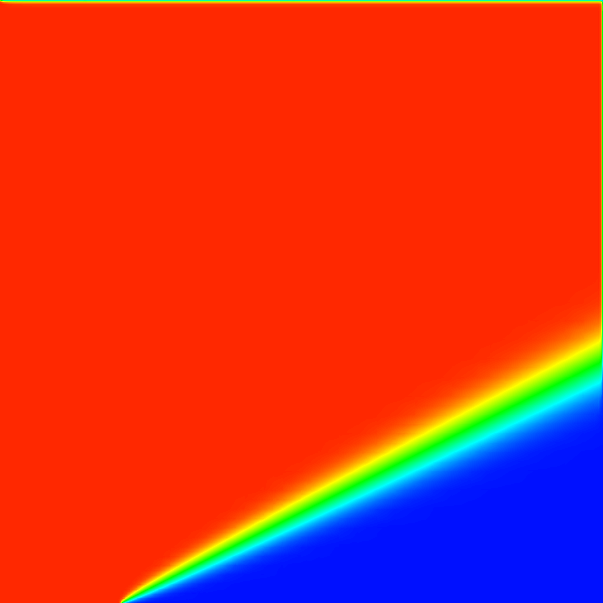
\includegraphics[scale = .175]{figs/Conservative/hughes.png}
}
\subfigure[Flow over a step]{
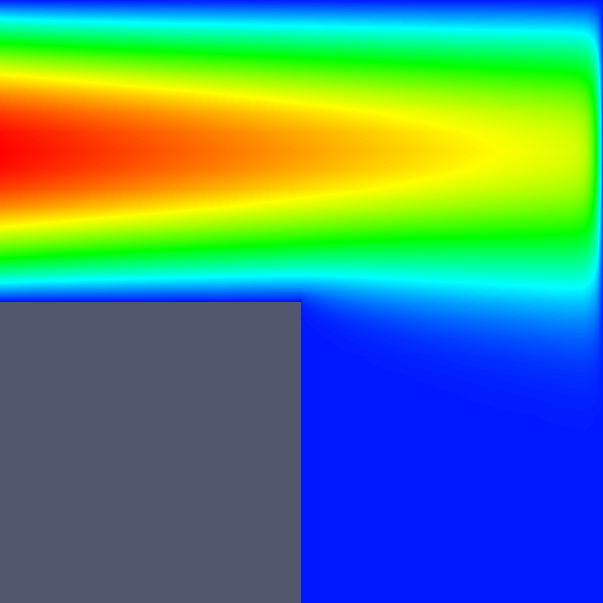
\includegraphics[scale = .175]{figs/Conservative/step.png}
}
\subfigure[Double glazing]{
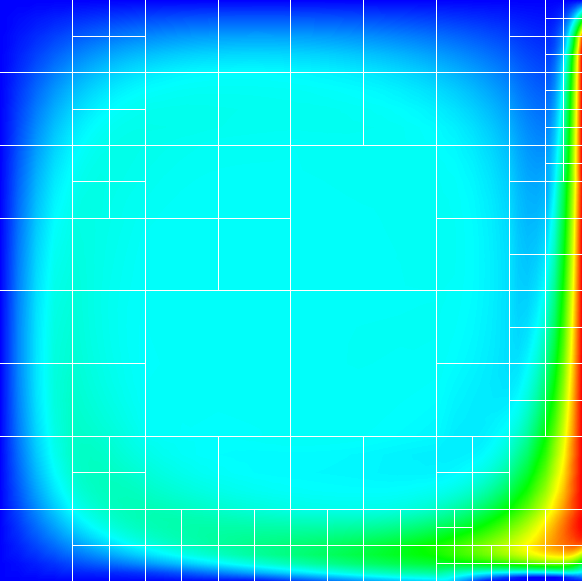
\includegraphics[scale = .182]{figs/Conservative/doubleGlazing.png}
}
\end{figure}
}

\frame{
\frametitle{Inviscid equations}
Issue: consider pure convection, $\div \beta u = f$. The ultra-weak variational formulation is
\[
\LRa{\widehat{f}_n,v}-\LRp{u,\beta\cdot \grad v} = \LRp{f,v},
\]
where $\widehat{f}_n \coloneqq \beta_n u$. When $\beta_n = 0$, $v$ has only a streamline derivative, and $\widehat{f}_n$ becomes an ill-defined trace in the cross-stream direction. For hyperbolic \emph{systems}, this issue manifests as \emph{sonic lines}. 
\begin{figure}
\centering
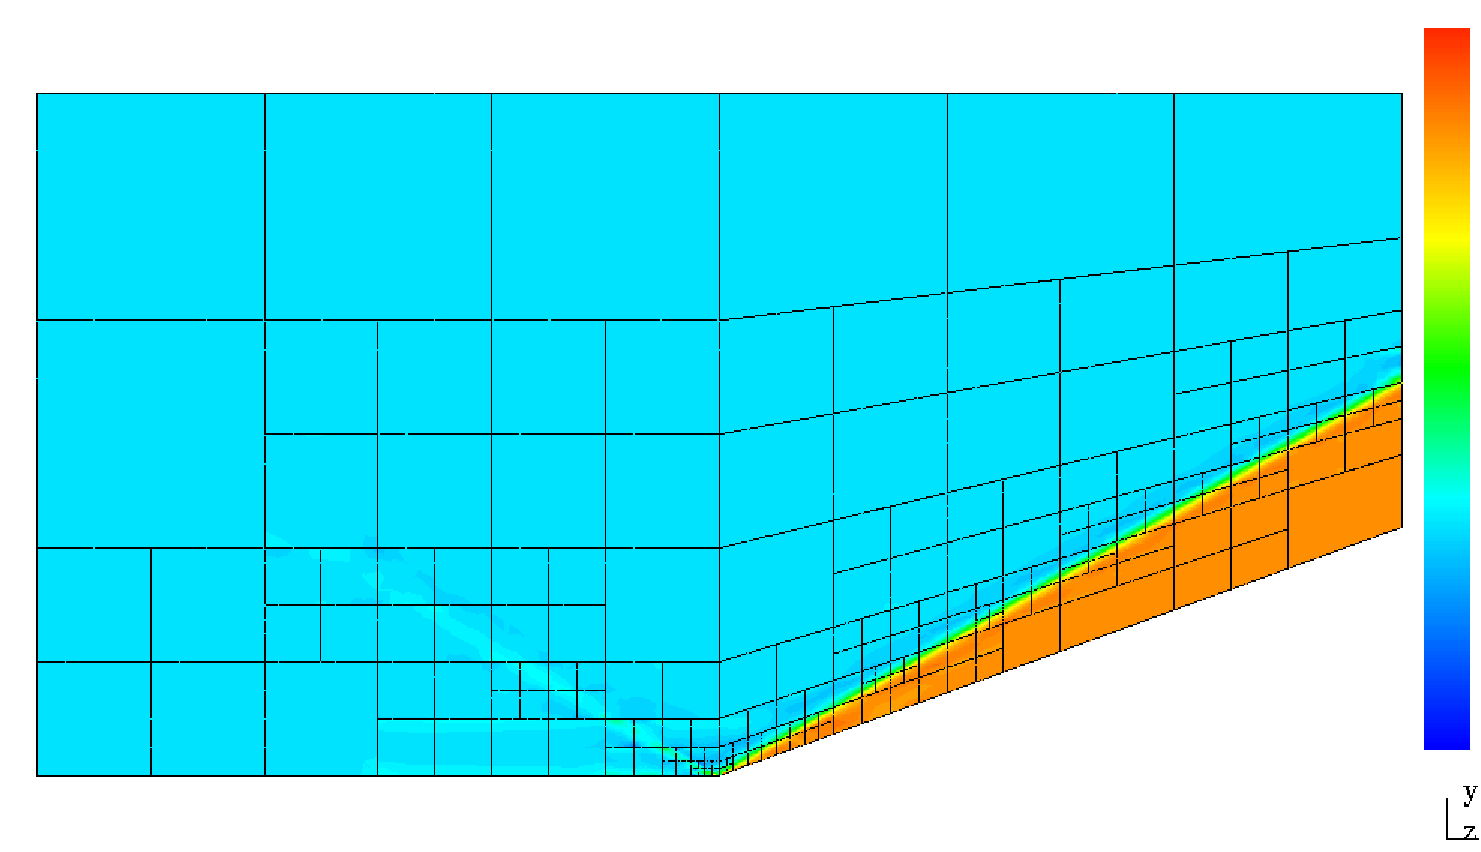
\includegraphics[scale=.25]{figs/sonicLines.pdf}
\caption{Sonic lines ($u_n - c = 0$) appear for linearized Euler.}
\end{figure}
}

\frame{
\frametitle{Regularization}
For $\beta = (-y,x)^T$ on $\Omega = [-1,1]^2$. Ill posed in the convection setting. Similar tests have been done with discontinuous data.

\begin{figure}
\centering
\subfigure{
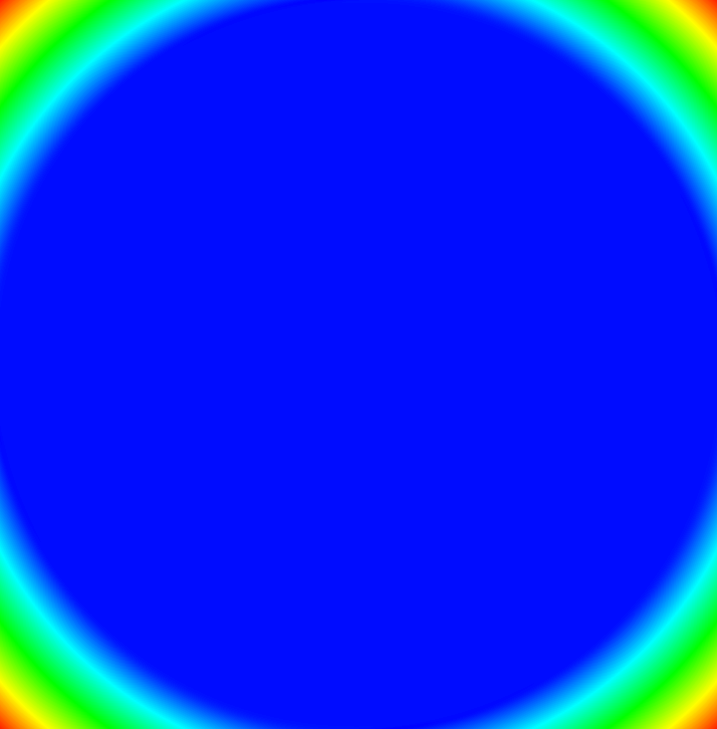
\includegraphics[scale=.21]{figs/vortex.png}
}
\subfigure{
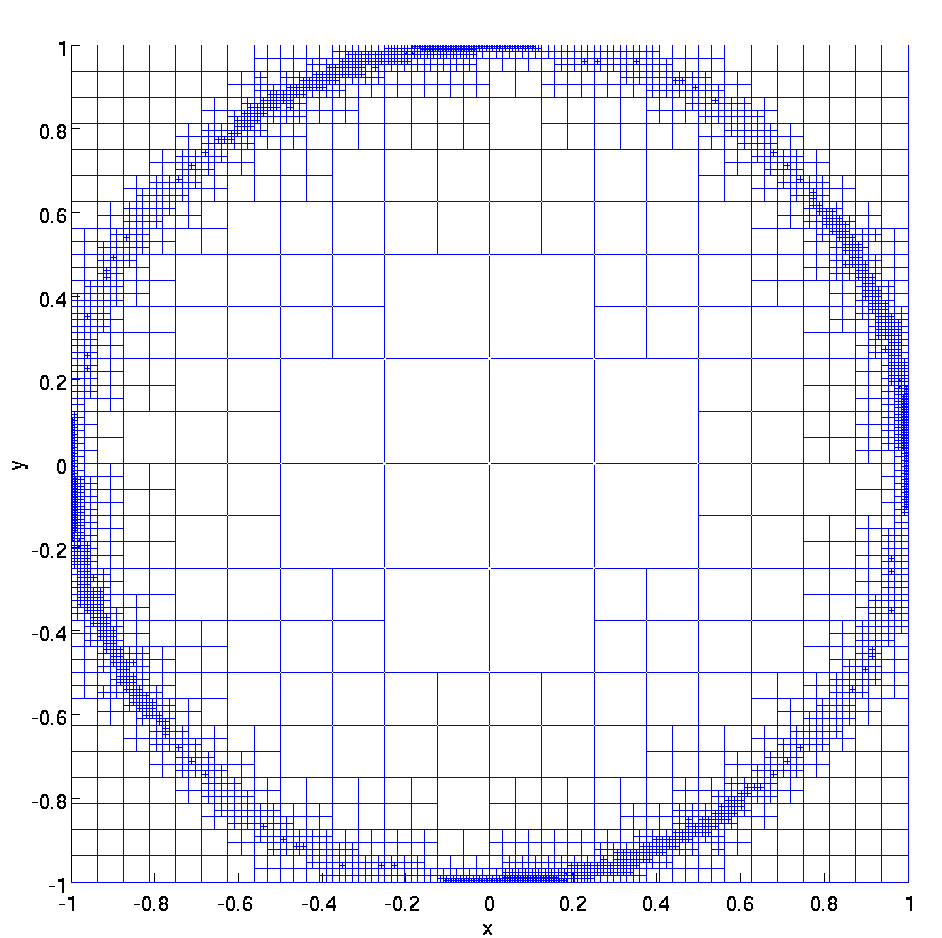
\includegraphics[scale=.2015]{figs/vortexMesh.png}
}
\caption{Steady vortex problem with $\epsilon = 1e-4$.}
\end{figure}
\vspace{-.25cm}
}

\frame{
\frametitle{Anisotropic refinement scheme}
}
